\section{Session and in-Session Experiments - Results} \label{sec:final-results}
From the results presented in previous sections of this chapter, we can fix now the packet level variables for all the tests, since their effect has been studied. The packet level configuration will be as follows:

\begin{itemize}
\item A uniform packet distribution with an average of 768 bytes [512 - 1024 bytes] for all flows and for all sessions.
\item An exponential packet inter-arrival time distribution with some practical mean [e.g. 100 ms] for all flows and for all sessions.
\end{itemize}

\subsection{Session Number Experiment} \label{sec:gv_session_exp}
First of all we tested the session level. For this, we used the following parametrization for the session number, e.g. the number of \acs{WLAN} terminals in the \acs{AP} area:

\begin{itemize}
	\item Low session number: \textbf{3 sessions}.
	\item Medium session number: \textbf{9 sessions}.
	\item High session number: \textbf{18 sessions}.
\end{itemize}

The three session cases have a similar load (25\%). With this experiment we want to test how the distribution of the load between different users affect the performance of the estimation and validation processes.

\begin{figure}[h!]
	\centering
	\subfloat[3 sessions]{
		\label{fig:3sessions}
		\includegraphics[width=0.33\textwidth]{images/results/GlobalView/sessions/3sessions}
	}
	\subfloat[9 sessions]{
		\label{fig:9sessions}
		\includegraphics[width=0.33\textwidth]{images/results/GlobalView/sessions/9sessions}
	}
	\subfloat[18 sessions]{
		\label{fig:18sessions}
		\includegraphics[width=0.33\textwidth]{images/results/GlobalView/sessions/18sessions}
	}
	\caption{Session number experiment - User realizations}
	\label{fig:user_realizations_final}
\end{figure}

All the sessions were configured to arrive at the same time, at the beginning of the simulation, representing that the users had been in the network for a while and then the sensor starts estimating. In real terms, the sensors can be off while the \acs{WLAN} network is working in order to improve their energy efficiency. The sensors could be activated once some sessions are already in the network transmitting data. For this experiment, the number of flows per session and its inter-arrival times have been fixed in the way that was done before. The packet level has been randomized with the configuration presented at the beginning of this sub-section. We run a total of 25 runs with the same configuration for each one of the three cases. Figure \ref{fig:user_realizations_final} represents the user realizations for each one of the three load cases under study in this experiment.

First of all, we need to check if the mixture idle distribution can still be used for the different traffic configurations that are under test. Figure \ref{fig:sessions_composed_cdf} represents the \acs{CDF} of the idle function for the three session cases.

\begin{figure}[h!]
	\centering
	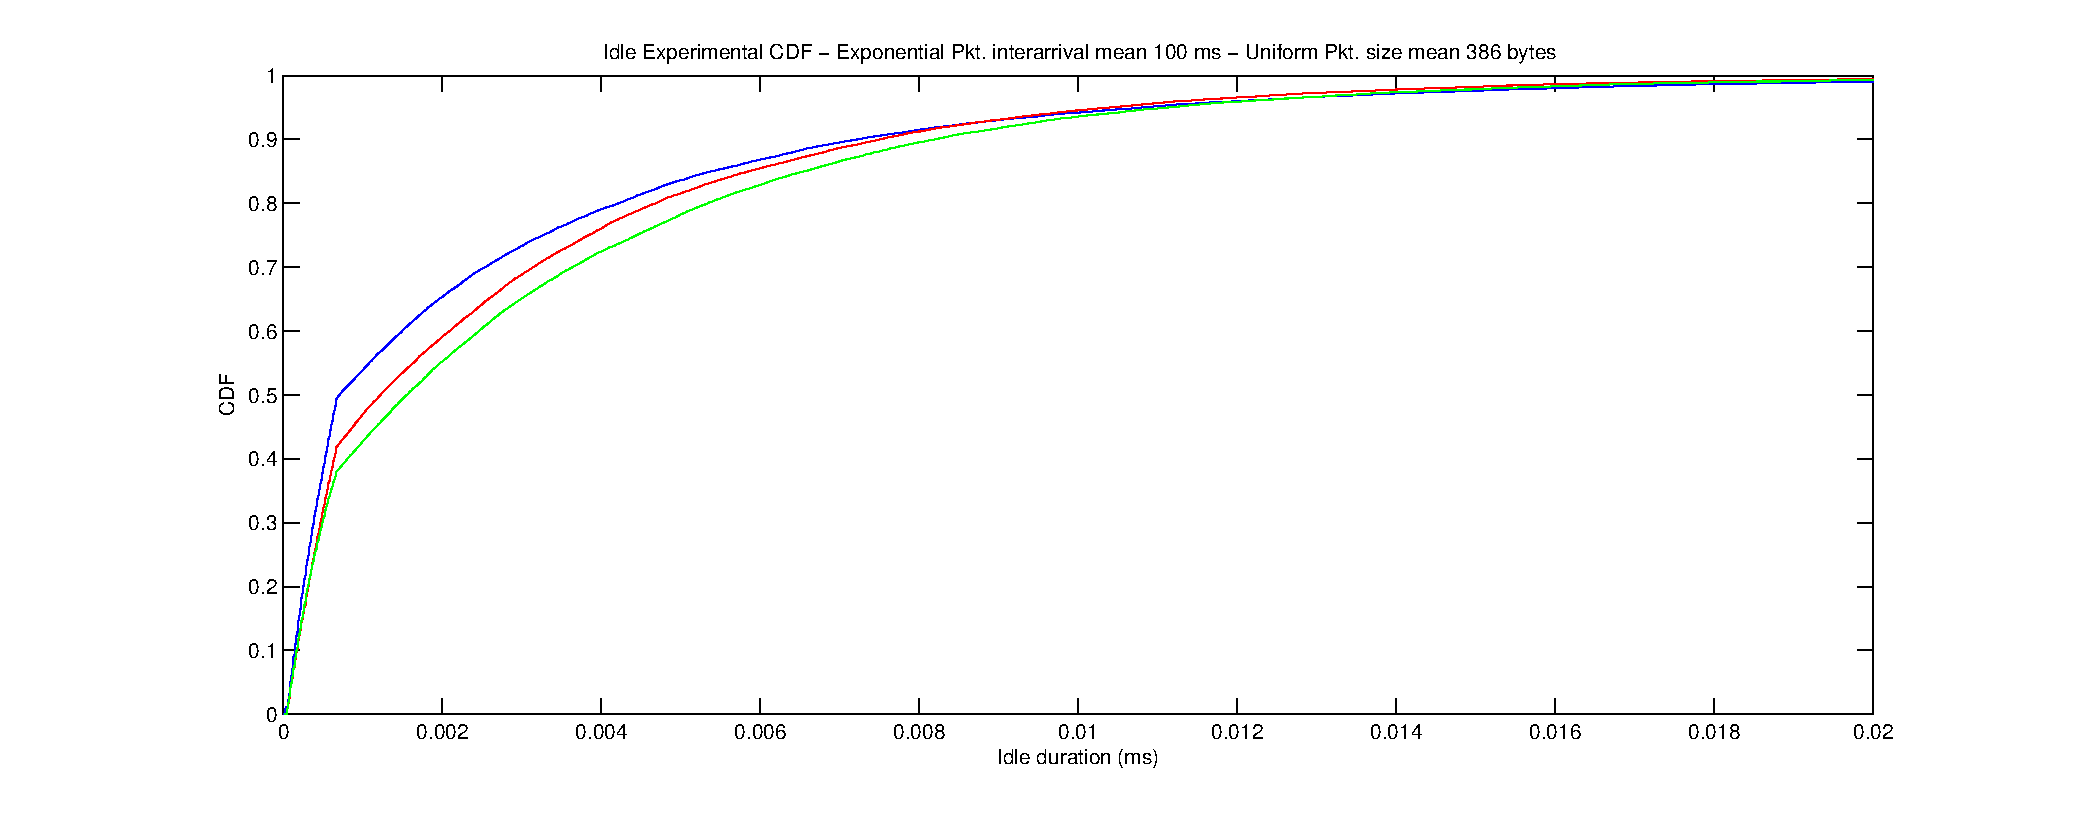
\includegraphics[width=0.9\textwidth]{images/results/GlobalView/sessions/sessions_composed_cdf}
	\caption{Idle distributions for different number of sessions}
	\label{fig:sessions_composed_cdf}
\end{figure}

As it can be observed in Figure \ref{fig:sessions_composed_cdf}, the mixture model can be used since two differentiated areas can be observed from the idle periods distribution as it has been shown previously.

Since the mixture model can be applied in the three scenarios, it is necessary to check if the estimation process and validation test are being carried properly. For this, we extracted the mean and standard deviation of the estimated parameters and the \acs{K-S} values for the 25 runs of each case. It can be observed from Table \ref{table:session_test}, that the variability of the estimated parameters and the \acs{K-S} values can be considered negligible.

\begin{table}[h!]
	\centering
	\begin{tabular}{ c | c | c || c | c || c | c }
		& \multicolumn{2}{ c || }{3 sessions} &  \multicolumn{2}{ c || }{9 sessions} & \multicolumn{2}{ c }{18 sessions}\\ \hline \hline
		& Mean & Std. Dev. & Mean & Std. Dev. & Mean & Std. Dev. \\ \hline
		$\xi$ & 0.184869 & 0.0109214 & 0.0639 & 0.0095 & 0.025 & 0.0097 \\ 
		$\sigma$ & 0.00337252 & 4.80725e-05 & 0.0036 & 5.9426e-05 & 0.0045 & 6.27E-005 \\
		$p$ & 0.38928 & 0.00444004 & 0.2996 & 0.0057 & 0.2397 & 0.004 \\
		$p_{KS}$ & 0.525856 & 0 0.253306 & 0.6874 & 0.2693 & 0.796 & 0.1874 \\ \hline
		$Fail$ & \multicolumn{2}{ c || }{0 \%} &  \multicolumn{2}{ c || }{0 \%} & \multicolumn{2}{ c }{0 \%}\\
	\end{tabular}
	\caption{Estimation parameters statistics for different number of sessions}
	\label{table:session_test}
\end{table}

The \acs{K-S} test shows that there are no fails for the three session-cases under study. The results presented in this section show that the distribution of the load between multiple \acs{WLAN} users do not affect the estimation and validation processes of the sensors. However, the results cannot be conclusive since are extracted from a 25-runs simulation. A higher numbers of runs are required to have statistically significant results.

\subsection{In-session statistics} \label{subsec:globalview_insession}
The following experiment randomizes what is happening at the flow level. This level describes the behavior of individual sessions, e.g. \acs{WLAN} users. For this experiment we tested different number of sessions representing different load regions. Following the traffic model defined in \cite{Campus-WLAN}, and the results obtained in this chapter, the different levels of the multi-layer traffic model has been configured as it is presented in Table \ref{tab:sim_traffic_model}. We randomized all the levels simultaneously in order to have multiple possible traffic scenarios in which to test the proposed model. The session cases under study in this these experiment are as follows:

\begin{itemize}
	\item 5 sessions - Standard traffic configuration.
	\item 5 sessions - Flow size magnified by 10.
	\item 10 sessions - Standard traffic configuration.
	\item 10 sessions - Flow size magnified by 10.
	\item 15 sessions - Standard traffic configuration. 
\end{itemize}

We decided to magnify the 5 and 10 session cases flow-sizes in order to achieve a higher load range for the same number of sessions but maintaining the distribution shape presented in Table \ref{tab:sim_traffic_model}. This magnification by 10 does not mean that the load will be 10 times higher than the standard configuration since the load is also affected by other parameters in the multi-layer traffic model such as flow number per sessions or packet sizes.

\begin{table}[h!]
	\begin{center}
		\begin{tabular}{ l | c | c }
			Modeled Variable & Distribution & Parameters \\ \hline
			Session number	& Fixed & N users arriving at simulator start \\
			Flow inter-arrival & Log-normal & $\mu = -1.6355$, $\sigma = 2.6286$ \\
			Flow number & Bi-Pareto & $\alpha = 0.07$, $\beta = 1.75$, $c = 295.38$, $k = 1$ \\
			Flow Size & Bi-Pareto & $\alpha = 0.00$, $\beta = 1.02$, $c = 15.56$, $k = 111$ \\
			Packet Size & Uniform & $min = 512$, $max = 1024$ \\
			Packet inter-arrival & Exponential & $\lambda = 10$ \\
		\end{tabular}
		\caption{The parameters used for generating traffic according to the model in \cite{Campus-WLAN}.}
		\label{tab:sim_traffic_model}
	\end{center}
\end{table}

We run 250 runs for each one of the five sub-experiments. For each run we extracted the D-value and P-value from the KS test and the load. The session level (number of sessions and inter-arrivals) will be fixed for all the runs of each sub-experiment while the flow and packet levels will be randomized following the distributions presented in Table \ref{tab:sim_traffic_model}.

Figure \ref{fig:insession_load_cdf} presents the \acs{CDF} of the loads for each one of the five experiments under study in this section. As it can be observed from the figure, the load is increased with the number of sessions. At the same time, for a same session case, the load also increases when the flow size is magnified. 

\begin{figure}[h!]
	\centering
	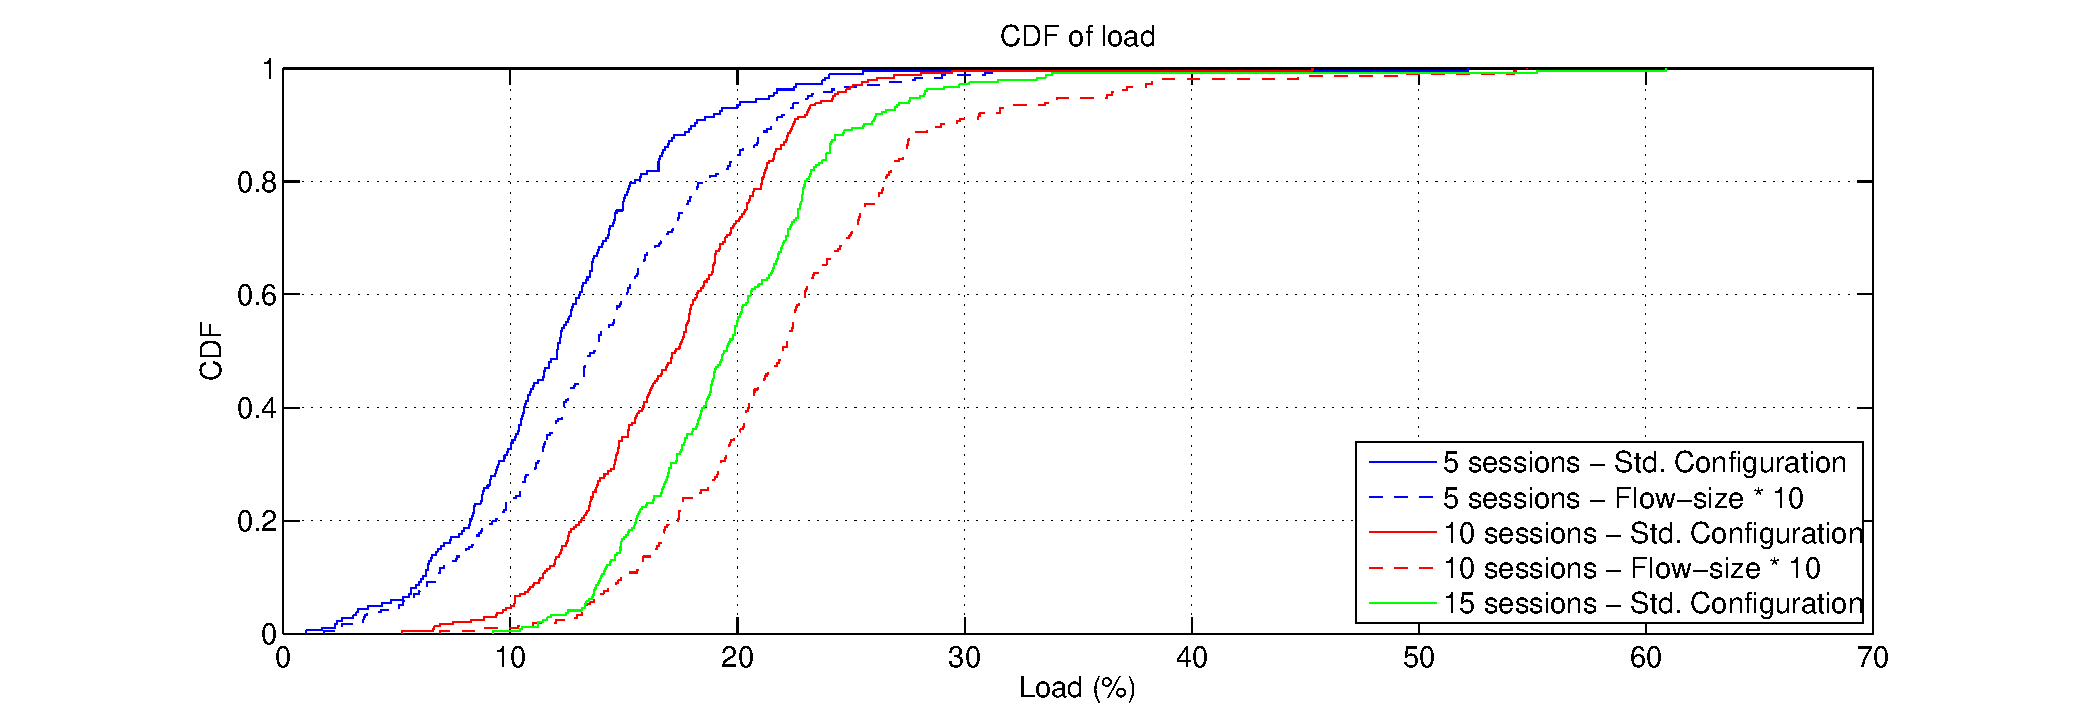
\includegraphics[width=0.9\textwidth]{images/results/GlobalView/flows/cdf_load}
	\caption{CDF of the loads for each one of the five experiments}
	\label{fig:insession_load_cdf}
\end{figure}

It can be observed that the load for all the experiments is concentrated around the 15 - 25 \% range. The mean load value for each experiment is presented in Table \ref{table:insession_mean_load}.

\begin{table}[h]
	\begin{center}
		\begin{tabular}{ l | c }
			Experiment & Load \\ \hline
			5 sessions - Standard Configuration & 12.202 \% \\
			5 sessions - Flow size * 10 & 14.0544 \% \\
			10 sessions - Standard Configuration & 17.1154 \% \\
			10 sessions - Flow size * 10 & 22.4922 \% \\
			15 sessions - Standard Configuration & 19.9669 \% \\
		\end{tabular}
		\caption{Average load for each one of the sub-experiments}
		\label{table:insession_mean_load}
	\end{center}
\end{table}

We represented the CDF of the d and p values from the KS test. This is represented in Figures \ref{fig:cdf_p_d}. As it can be observed the P-value is almost equally distributed for all the experiments (Figure \ref{fig:insession_cdf_p}), with a failure rate of around 5 \% for all the cases. On the other hand, in Figure \ref{fig:insession_cdf_d} it can be observed that the D-value is clearly improved when the load is higher.

\begin{figure}[h!]
	\centering
	\subfloat[P-value]{
		\label{fig:insession_cdf_p}
		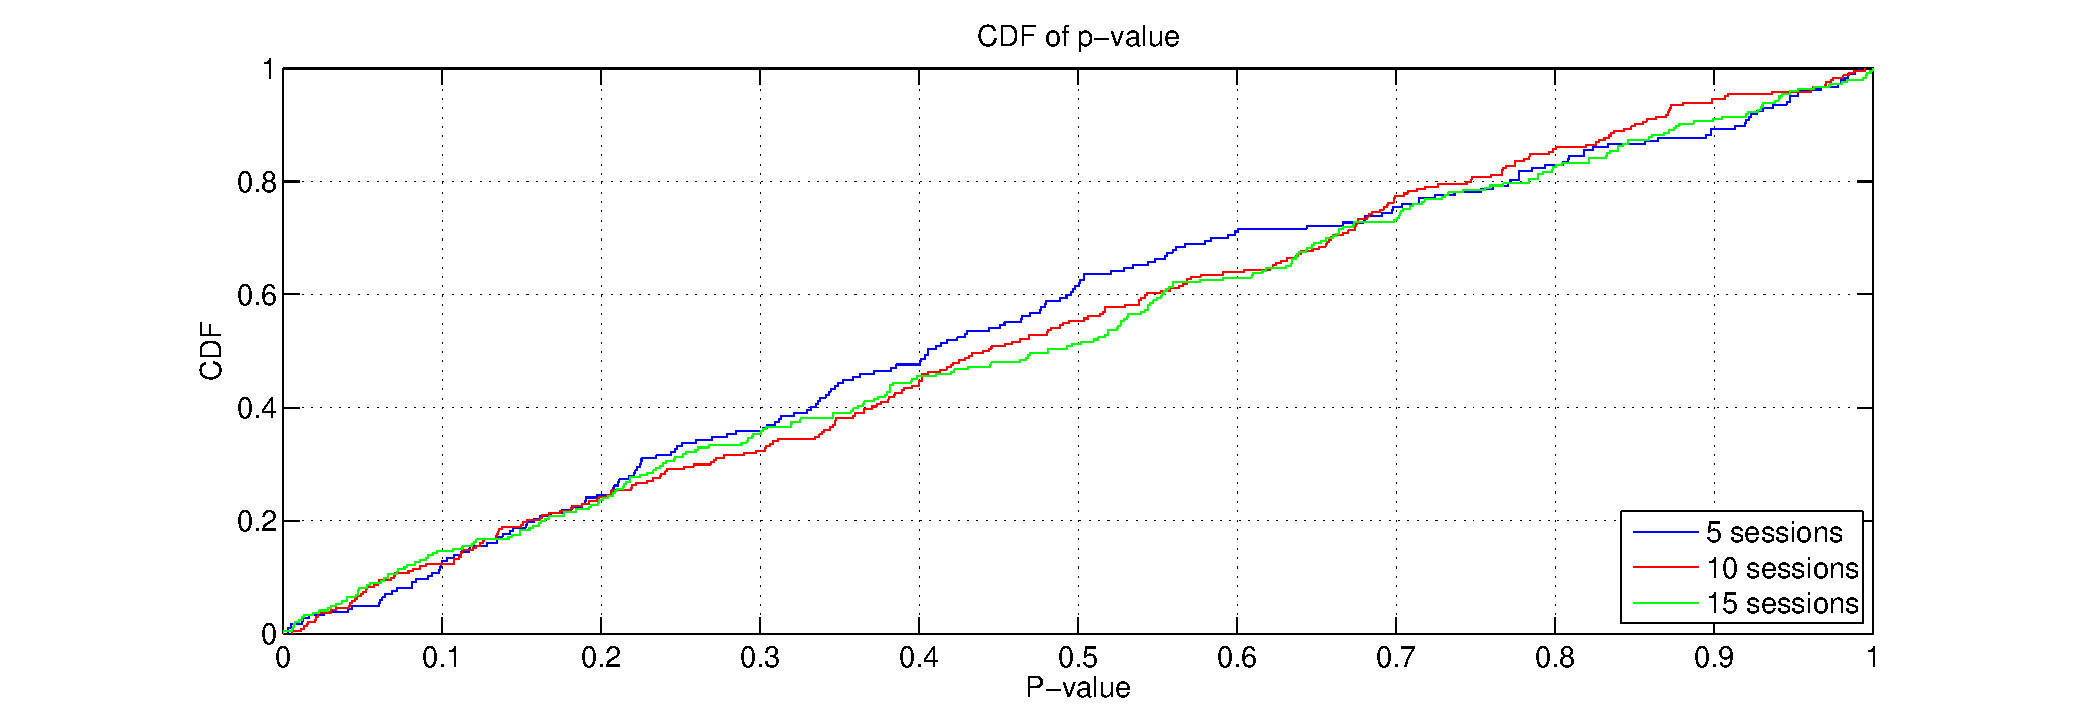
\includegraphics[width=0.9\textwidth]{images/results/GlobalView/flows/cdf_p}
	}\\
	\subfloat[D-value]{
		\label{fig:insession_cdf_d}
		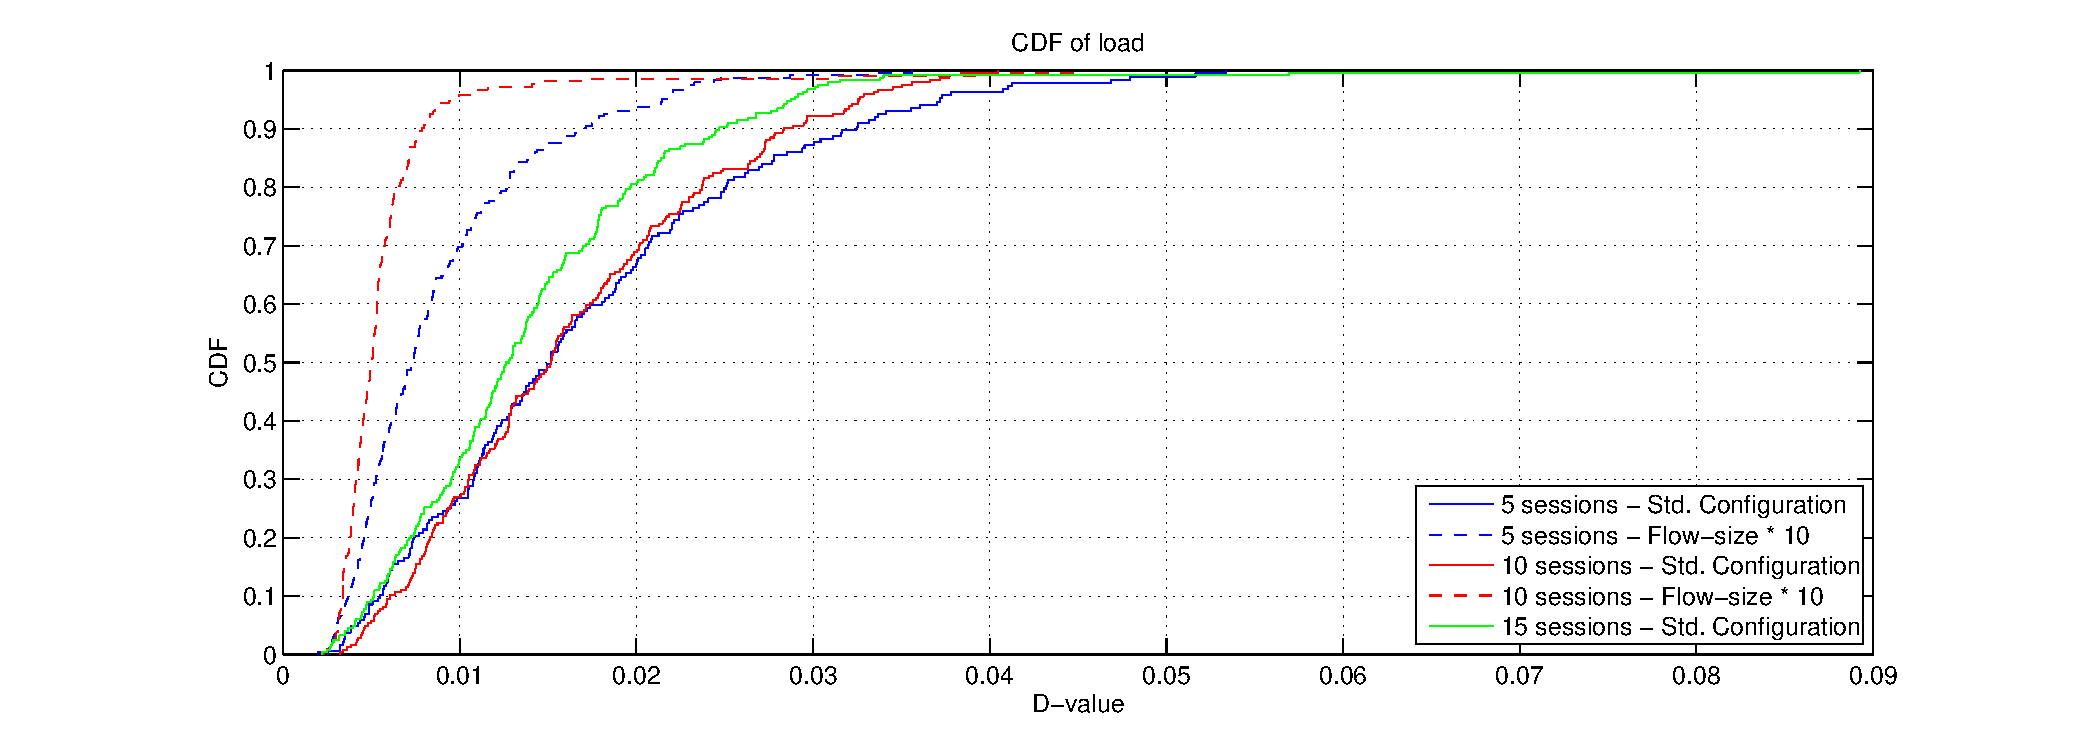
\includegraphics[width=0.9\textwidth]{images/results/GlobalView/flows/cdf_d}
	}
	\caption{CDF of P-value and D-value from the KS test for each experiment}
	\label{fig:cdf_p_d}
\end{figure}

Our main goal in this project is to determine when our model can be used. In order to have a better insight on how the model behaves, we filtered the results in different load regions to study how the p and d values are affected. Figure \ref{fig:insession_regions_n_tests} represents the number of tests for each region (aggregate from all the five experiments). As it can be observed, a big amount of the tests are concentrated in the region of 10 to 25 \% load region (this also can be observed in Figure \ref{fig:insession_load_cdf}).

\begin{figure}[h!]
	\centering
	\includegraphics[width=0.9\textwidth]{images/results/GlobalView/flows/n_tests}
	\caption{Number of tests per load region (aggregate from all the experiments)}
	\label{fig:insession_regions_n_tests}
\end{figure}

We represented the mean p value for each one of the load regions for each sub-experiment in Figure \ref{fig:insession_p_regions}. The most significant results are represented in the load region where all the tests are concentrated (from 10 to 25 \% of load). In this region, the mean p-value is almost the same for the five experiments, which means that it is not affected by the number of sessions. The rest of the regions represent a small amount of tests, this is why the difference between the p-values is really high between the experiments. In order to have a higher number of tests in each region, we plotted the aggregate mean p-value for all the tests (Figure \ref{fig:insession_mean_p_all}). It can be observed how the p-value is approximately the same for each one of the regions, even so, we may need a higher number of runs of each experiment to have a better conclusion.

\begin{figure}[h!]
	\centering
	\subfloat[5 experiments]{
		\label{fig:insession_mean_p}
		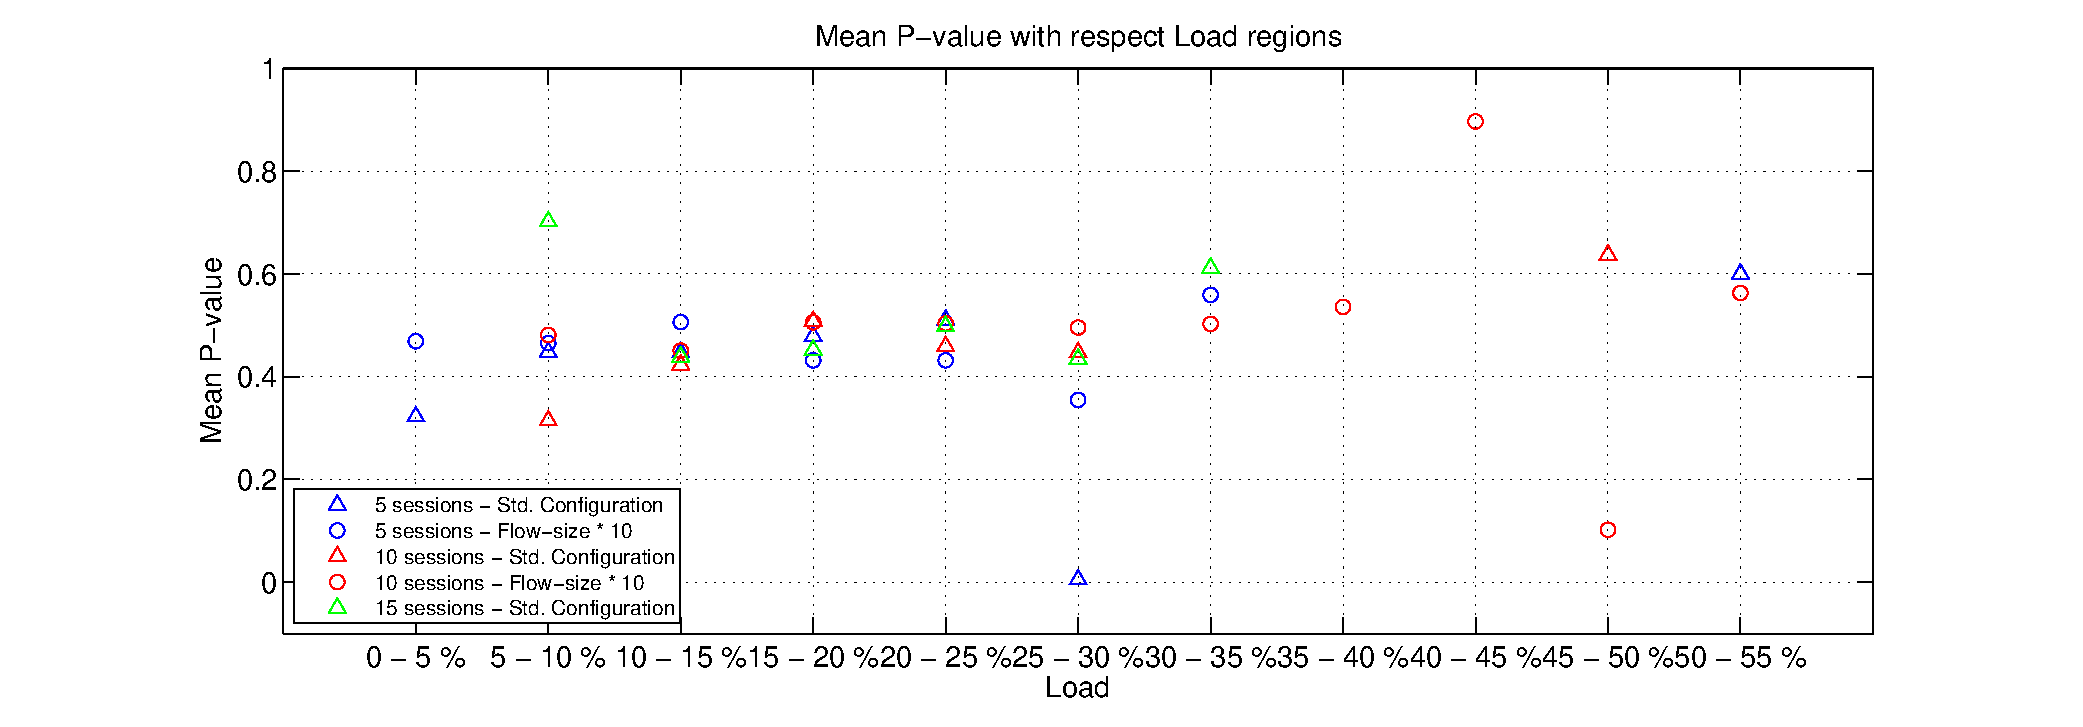
\includegraphics[width=0.9\textwidth]{images/results/GlobalView/flows/load_vs_p}
	}\\
	\subfloat[Aggregate]{
		\label{fig:insession_mean_p_all}
		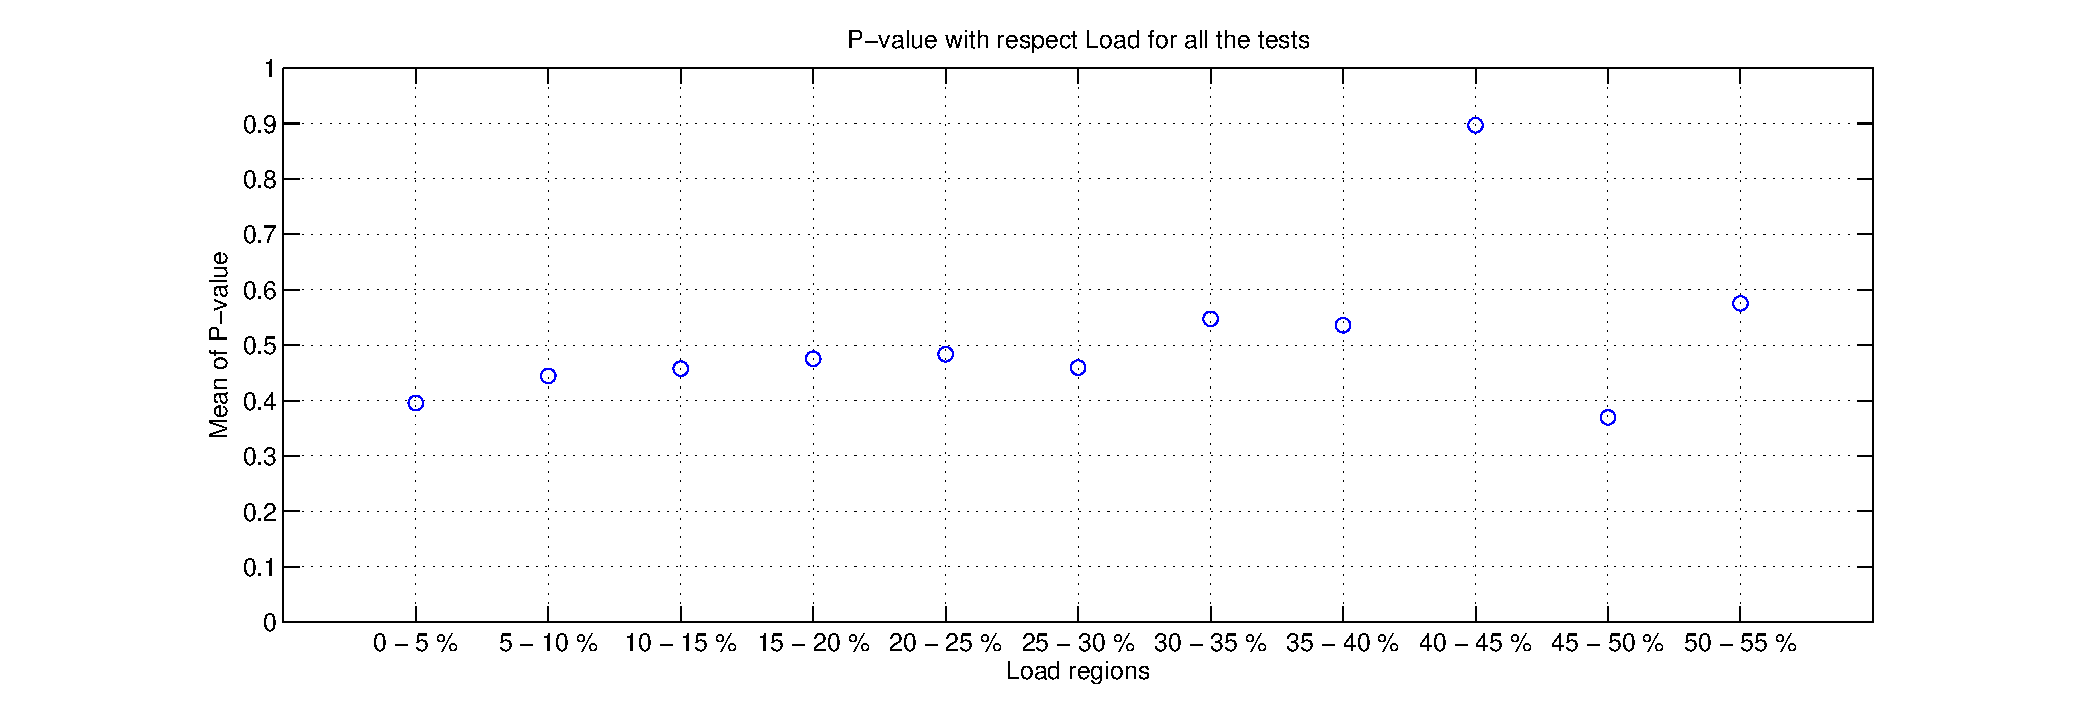
\includegraphics[width=0.9\textwidth]{images/results/GlobalView/flows/load_vs_p_all}
	}
	\caption{Mean P-value for the different load regions}
	\label{fig:insession_p_regions}
\end{figure}

We did the same for the d value as it is represented in Figure \ref{fig:insession_d_regions}. In this case, we have a similar behaviour as the presented in the p-value results. The variability between experiments is low enough to be considered null in the load regions with higher concentration of tests.

\begin{figure}[h!]
	\centering
	\subfloat[5 experiments]{
		\label{fig:insession_mean_p}
		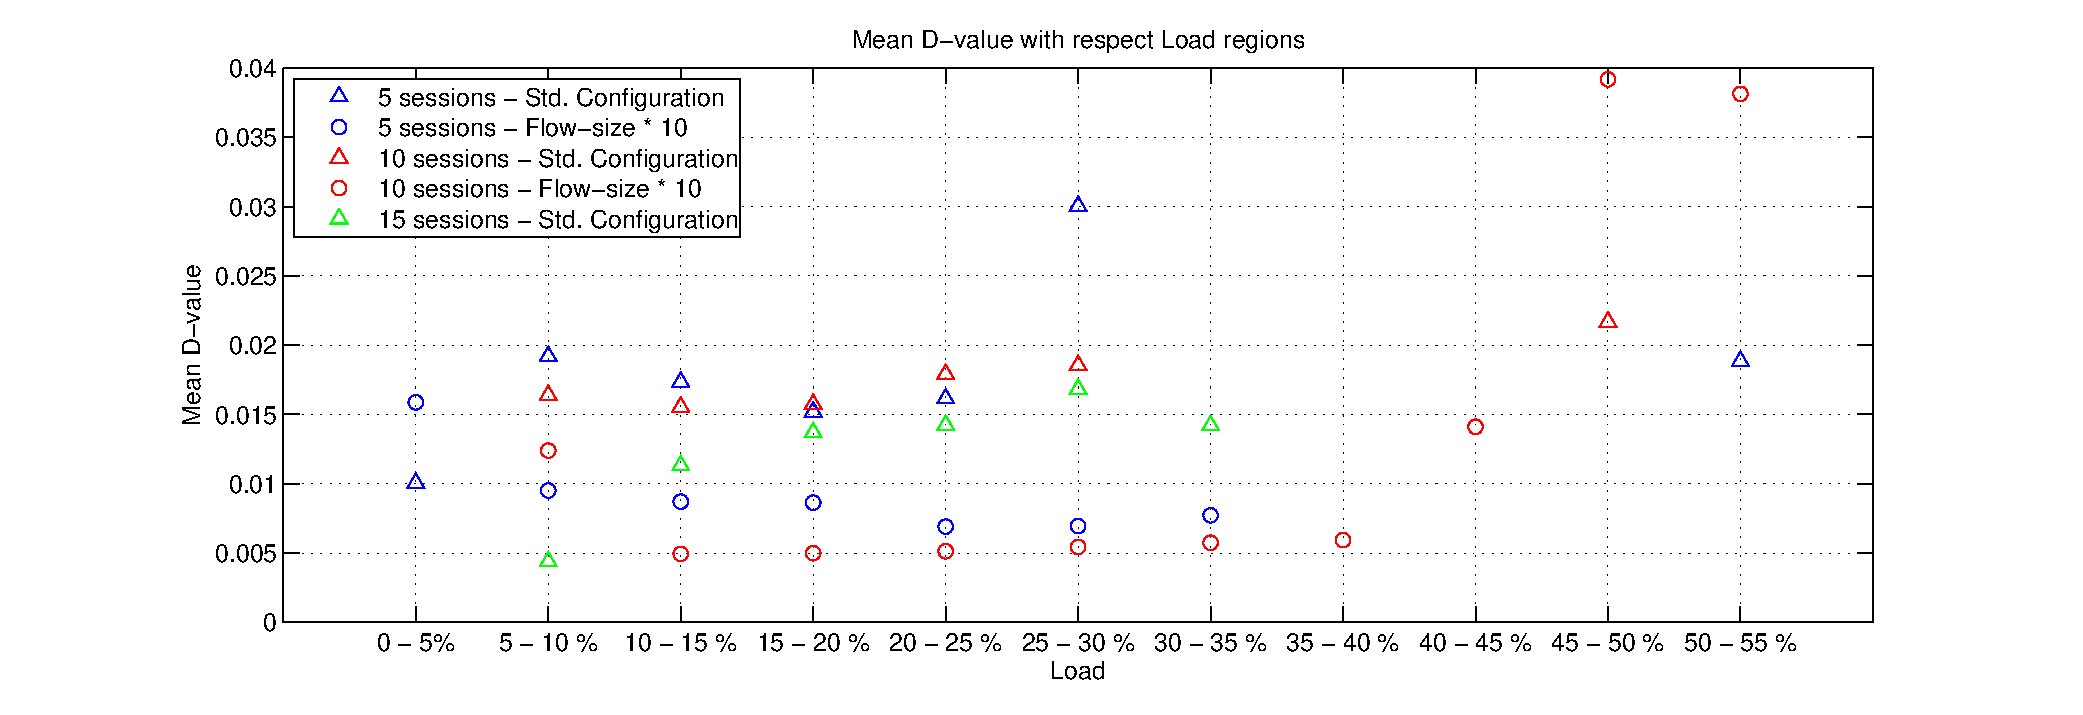
\includegraphics[width=0.9\textwidth]{images/results/GlobalView/flows/load_vs_d}
	}\\
	\subfloat[Aggregate]{
		\label{fig:insession_mean_p_all}
		\includegraphics[width=0.9\textwidth]{images/results/GlobalView/flows/load_vs_d_all}
	}
	\caption{Mean D-value for the different load regions}
	\label{fig:insession_d_regions}
\end{figure}

From the results presented, we can conclude that our model can be applied for different session cases in the region of 10 - 30 \% of load, achieving a low failure rate in the KS test and similar results between different number of sessions. On the other hand, an extended study of lower and higher load regions is needed in order to determine how our model works in those cases.